% !TEX root = main.tex

\newgeometry{top=2.170cm,
            bottom=3.510cm,
            inner=2.1835cm,
            outer=2.1835cm,
            ignoremp}


%\begin{titlepage}
%   \begin{center}
%       \vspace*{4cm}

 %      \textbf{\Huge Improved microfading device for risk assessment of colour change in Van Gogh's works}

           
%       \vspace{7cm}

 %      \textbf{\Large Gauthier Patin}          
  
            
  % \end{center}
%\end{titlepage}




% Copyright page




%\clearpage
%\thispagestyle{empty}
\null%
\label{thesis:colophon}
\vfill
\pdfbookmark[1]{Colophon}{thesis:colophon}
Written in 2018--2023 by Gauthier Patin 

ISBN: 978909037535

Copyright \copyright \hspace{0.1cm}2023 by Gauthier Patin

Printed by Proefschriftmaken, \url{https://www.proefschriftmaken.nl}\\


\textbf{Caveat} \\
I must note that throughout this thesis I have used several excerpts of others' text, images and code, which I have always been careful to mark as such.
While I am allowed to use these excerpts under legal \emph{fair use} doctrines in many countries and more specifically by the citation right (\emph{citaatrecht}) in \href{http://wetten.overheid.nl/jci1.3:c:BWBR0001886&hoofdstuk=I&paragraaf=6&artikel=15a&z=2015-07-01&g=2015-07-01}{Article 15a of the Dutch Copyright Law} (\emph{Auteurswet}), it does not follow that you are also free to use these excerpts for any purpose.\\

\textbf{Colophon} \\
This thesis was typeset with the help of \LaTeX{} and to a large extent uses the source code provided by Ken Arroyo Ohori for his PhD thesis (\url{https://github.com/kenohori/thesis}). Most of the figures were created using Matplotlib package inside Jupyter notebooks, or Inkscape.

The source code of this thesis is available at: \url{https://github.com/g-patin/PhD_thesis}

A digital version of this dissertation is available on the Digital Academic Repository of the University of Amsterdam (\url{https://dare.uva.nl}) as well on my PhD website (\url{https://microfadingphd.wordpress.com}). 

The data that have been used to create the figures in Chapters 3, 4, and 5 have been stored on a Zenodo repository (\url{https://zenodo.org/record/8216110}). \\

\textbf{Cover} \\
The front and back covers are based on the results of light ageing experiments conducted during this PhD using the methodology described in Chapter 4 (section \ref{sec:DL_methodology}) of this dissertation. Both covers display the results of daylight exposure on an eosin paint-out (PO098). The front cover shows visualization of colour patches as the light dose increases from 0 to 120 MJ/m\textsuperscript{2}, while the back cover shows differences in the reflectance spectra as the light dose increases from 0 to 120 MJ/m\textsuperscript{2}. A value of 120 MJ/m\textsuperscript{2} roughly corresponds to 50 years of continuous exposure in the galleries of the Van Gogh Museum (10 hours per day at 50 lux).




% Official title
%\begin{titlepage}
%\begin{center}
%    \vspace*{3cm}

%    \textbf{\Large Improved microfading device}\\
%    \vspace{1cm}
%    \textbf{\Large for risk assessment of colour change}\\
%    \vspace{1cm}
%    \textbf{\Large in Van Gogh's works}

           
%    \vspace{4cm}
    

%% Skip space as in half-title
%\vspace*{4\baselineskip}



%{\Large ACADEMISCH PROEFSCHRIFT}

%\medskip
%\large
%{ter verkrijging van de graad van doctor aan de Universiteit van Amsterdam \\
%op gezag van de Rector Magnificus \\
%prof. dr. ir. P.P.C.C. Verbeek \\
%ten overstaan van een door het College voor promoties ingestelde commissie, \\
%in het openbaar te verdedigen op vrijdag XX XXXX 2024, te XX:00 uur \\
%}

%\medskip

%door

%\medskip

%% Print the full name of the author.
%\makeatletter
%{\Large Gauthier {\scshape Patin}}
%\makeatother

%\medskip

%geboren te Grande-Synthe, Frankrijk.

%\end{center}
%\end{titlepage}


% Official verso
%\clearpage
%\thispagestyle{empty}
%\null%
%\label{thesis:committee}
%\vfill
%\pdfbookmark[1]{Doctoral committee}{thesis:committee}

\afterpage{\blankpage}
\newpage
{\Large\textbf{Promotiecommissie}}

\vspace{1cm}


\medskip\noindent
\begin{tabular}{@{}lll@{}}
  Promotor: & prof.\ dr.\ E.\ Hendriks &  Universiteit van Amsterdam\\
  & & \\
  Copromotores: & prof.\ dr.\ K.J.\ van den Berg &  Universiteit van Amsterdam\\  
  & prof.\ dr.\ R.G.\ Erdmann &  Universiteit van Amsterdam\\
  & & \\
  Overige leden: & prof.\ dr.\ M.R.\ van Bommel & Universiteit van Amsterdam \\  
  & prof.\ dr.\ S.\ Woutersen & Universiteit van Amsterdam \\
  & prof.\ dr.\ K.\ Keune & Universiteit van Amsterdam  \\  
  & prof.\ dr.\ S.\ Woutersen & Universiteit van Amsterdam \\
  & prof.\ dr.\ J.\ Dik & TU Delft \\
  & dr.\ J.\ del Hoyo-Meléndez & National Museum Krakow \\
  & dr.\ A.\ Bülow & Stedelijk Museum Amsterdam\\
\\

\end{tabular}

\vspace{0.5cm}
Faculteit der Geesteswetenschappen



\newpage

{\Large\textbf{Funding}}\\

The research for this thesis received financial assitance from the AXA Research Fund, the Van Gogh Museum-ASML Partnership in Science, the Rijksdienst voor het Cultureel Erfgoed, and the Rijksmuseum Amsterdam. 

\vspace{1.5cm}

\begin{figure}[!h]
\centering
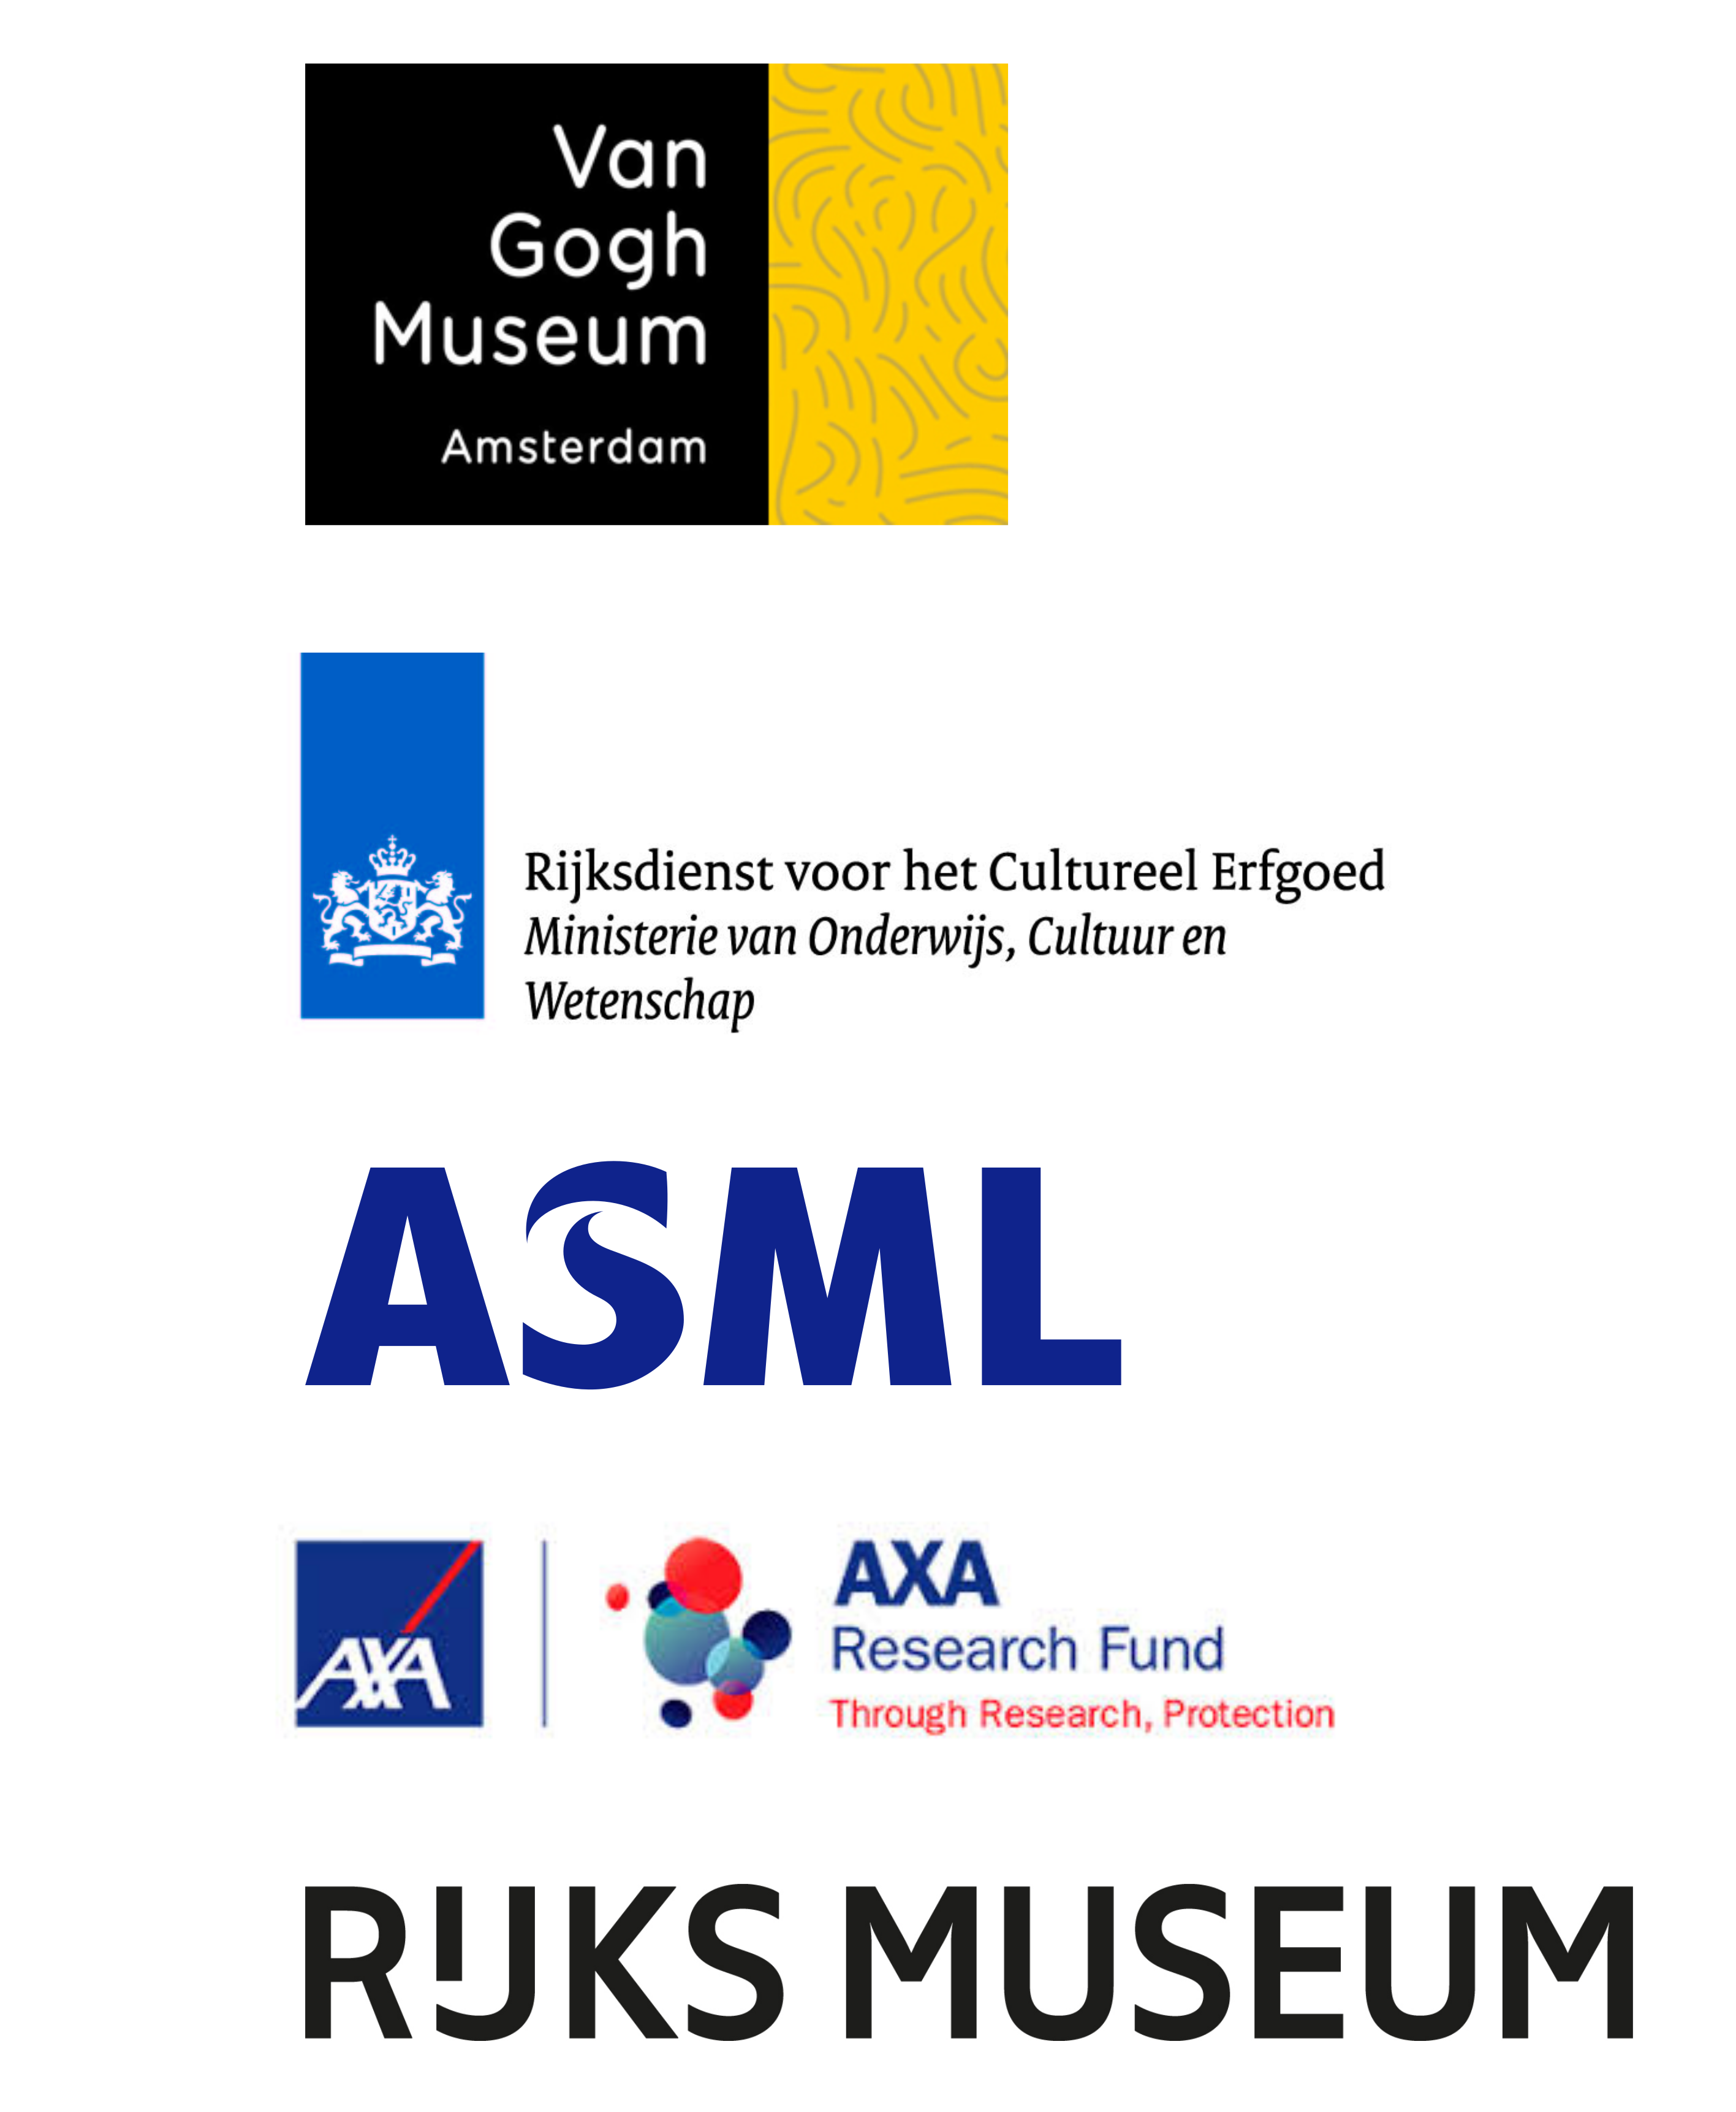
\includegraphics[width=0.75\textwidth]{Logo_institutions.png}
\label{fig:colours_description}
\end{figure}

\newpage
